\documentclass[tikz,border=5pt]{standalone}
\usepackage{xcolor}
\usepackage{tikz}
\usetikzlibrary{arrows.meta,positioning}
\usetikzlibrary{calc}

\begin{document}
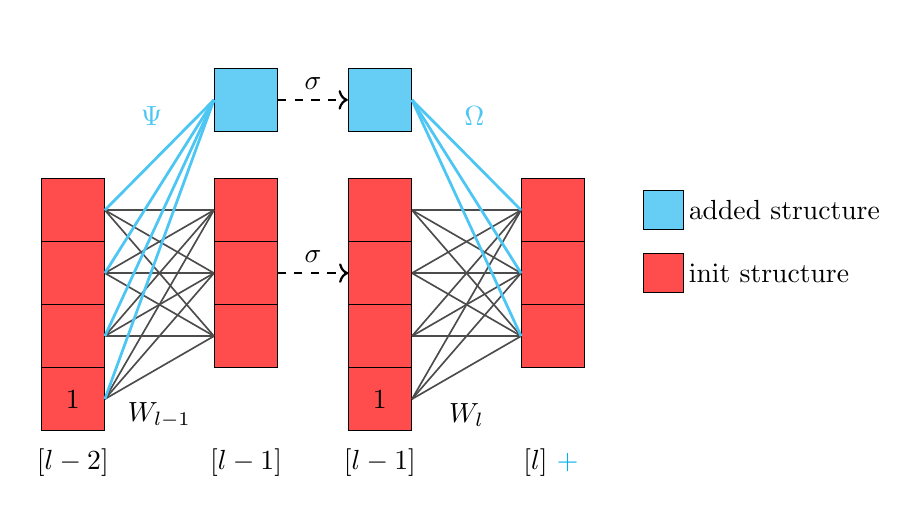
\begin{tikzpicture}[
    neuron/.style={draw, rectangle, minimum width=8mm, minimum height=8mm},
    redneuron/.style={neuron, fill=red!70},
    blueneuron/.style={neuron, fill=cyan!60},
    conn/.style={-, black!70, line width=0.6pt},
    addconn/.style={-, cyan!70, line width=1pt},
    act/.style={->, dashed, line width=0.8pt}
]

% x positions of layers
\def\xA{0}
\def\xB{2.2}
\def\xC{3.9}
\def\xD{6.1}

% Layer A (h_{l-2}(x))
\foreach \i in {0,...,2} {
    \node[redneuron] (A\i) at (\xA, \i*0.8) {};
}
\node[redneuron] (Aone) at (\xA,-0.8) {1};

\node at (\xA,-1.6) {$\postact[l-2]$};

% Layer B (z_{l-1}(x))
\foreach \i in {0,...,2} {
    \node[redneuron] (B\i) at (\xB, \i*0.8) {};
}
\node at (\xB,-1.6) {$\preact[l-1]$};

% Layer C (h_{l-1}(x))
\foreach \i in {0,...,2} {
    \node[redneuron] (C\i) at (\xC, \i*0.8) {};
}
\node[redneuron] (Cone) at (\xC,-0.8) {1};

\node at (\xC,-1.6) {$\postact[l-1]$};

% Layer D (z_l(x))
\foreach \i in {0,...,2} {
    \node[redneuron] (D\i) at (\xD, \i*0.8) {};
}
\node at (\xD,-1.6) {$\preact[l]$ \textcolor{cyan!100}{$ + \,\deltas$}};

% Added blue neurons (top)
\node[blueneuron] (Badd) at (\xB,3) {};
\node[blueneuron] (Cadd) at (\xC,3) {};

% Activation arrows
\draw[act] (Badd) -- node[above] {$\sigma$} (Cadd);
\draw[act] ($(B1)+(0.4, 0)$) -- node[above] {$\sigma$} ($(C1)-(0.4, 0)$);

% Dense connections A -> B
\foreach \i in {0,...,2} {
    \foreach \j in {0,...,2} {
        \draw[conn] (A\i.east) -- (B\j.west);
    }
}
\foreach \j in {0,...,2} {
    \draw[conn] (Aone.east) -- (B\j.west);
}

% Dense connections C -> D
\foreach \i in {0,...,2} {
    \foreach \j in {0,...,2} {
        \draw[conn] (C\i.east) -- (D\j.west);
    }
}
\foreach \j in {0,...,2} {
    \draw[conn] (Cone.east) -- (D\j.west);
}

% Added cyan connections A -> Badd
\foreach \i in {0,...,2} {
    \draw[addconn] (A\i.east) -- (Badd.west);
}
\draw[addconn] (Aone.east) -- (Badd.west);

% Added cyan connections Cadd -> D
\foreach \j in {0,...,2} {
    \draw[addconn] (Cadd.east) -- (D\j.west);
}

% Labels
\node at (\xB-1.1,-1) {$W_{l-1}$};
\node[cyan!70] at (\xB-1.2,2.8) {$\Psi$};
\node[cyan!70] at (\xC+1.2,2.8) {$\Omega$};
\node at (\xD-1.1,-1) {$W_l$};

\node[cyan!70] at (\xB,3.8) {\textcolor{cyan!100}{$\preactext$}};
\node[cyan!70] at (\xC,3.8) {\textcolor{cyan!100}{$\postactext$}};

% Legend (right side)
\node[blueneuron, minimum width=5mm, minimum height=5mm] at (7.5, 1.6) {};
\node[anchor=west] at (7.7, 1.6) {added structure};

\node[redneuron, minimum width=5mm, minimum height=5mm] at (7.5, 0.8) {};
\node[anchor=west] at (7.7, 0.8) {init structure};

\end{tikzpicture}
\end{document}